\documentclass[pstricks,14 pt]{extarticle}

	\usepackage[frenchb]{babel}
	\usepackage[utf8]{inputenc}  
	\usepackage[T1]{fontenc}
	\usepackage{amssymb}
	\usepackage[mathscr]{euscript}
	\usepackage{stmaryrd}
	\usepackage{amsmath}
	\usepackage{tabularx} 
	\usepackage{pstricks}
	\usepackage{pst-all} 
	\usepackage{tikz}
	\usepackage[all,cmtip]{xy}
	\usepackage{amsthm}
	\usepackage{varioref}
	\usepackage{geometry}
	\geometry{a4paper}
	\usepackage{lmodern}
	\usepackage{hyperref}
	\usepackage{array}
	 \usepackage{fancyhdr}
\usepackage{pstricks-add,multido}
	 \usepackage{float}
\renewcommand{\theenumi}{\alph{enumi})}
	\pagestyle{fancy}
	\theoremstyle{plain} 
	\fancyfoot[C]{} 
	\fancyhead[L]{Contrôle}
	\fancyhead[R]{Géométrie dans l'espace}\geometry{
 a4paper,
 total={170mm,257mm},
 left=10mm,
 right=10mm,
 top=18mm,
 bottom = 10mm
 }
	
	
	\title{Contrôle }
	\date{}
	\begin{document} 
\subsection*{Exercice 1 - 6 points}	%(1 + 2 + 2 + 1)  
Réduire les expressions suivantes : 
\begin{enumerate}
\item $(3x+1) + (x+3)$
\item $(3x+1)(x+3)$
\end{enumerate}
Combien valent : \begin{enumerate}
\item un prix de $15$ euros après une augmentation de $10\%$.
\item le prix initial d'un objet valant $36$ euros après avoir augmenté de
$20\%$. 
\end{enumerate}

\subsection*{Exercice 2 (0,5+2+2+1+2+2) =9,5 points }  % 1+ 2 + 2+ 1 +2  + 2

M. et M\up{me} Martin veulent construire une terrasse en béton dans leur jardin. Ils souhaitent que leur terrasse ait une hauteur de $15 \mathrm{~cm}$. Les représentations ci-dessous ne sont pas à l'échelle.


\begin{center}
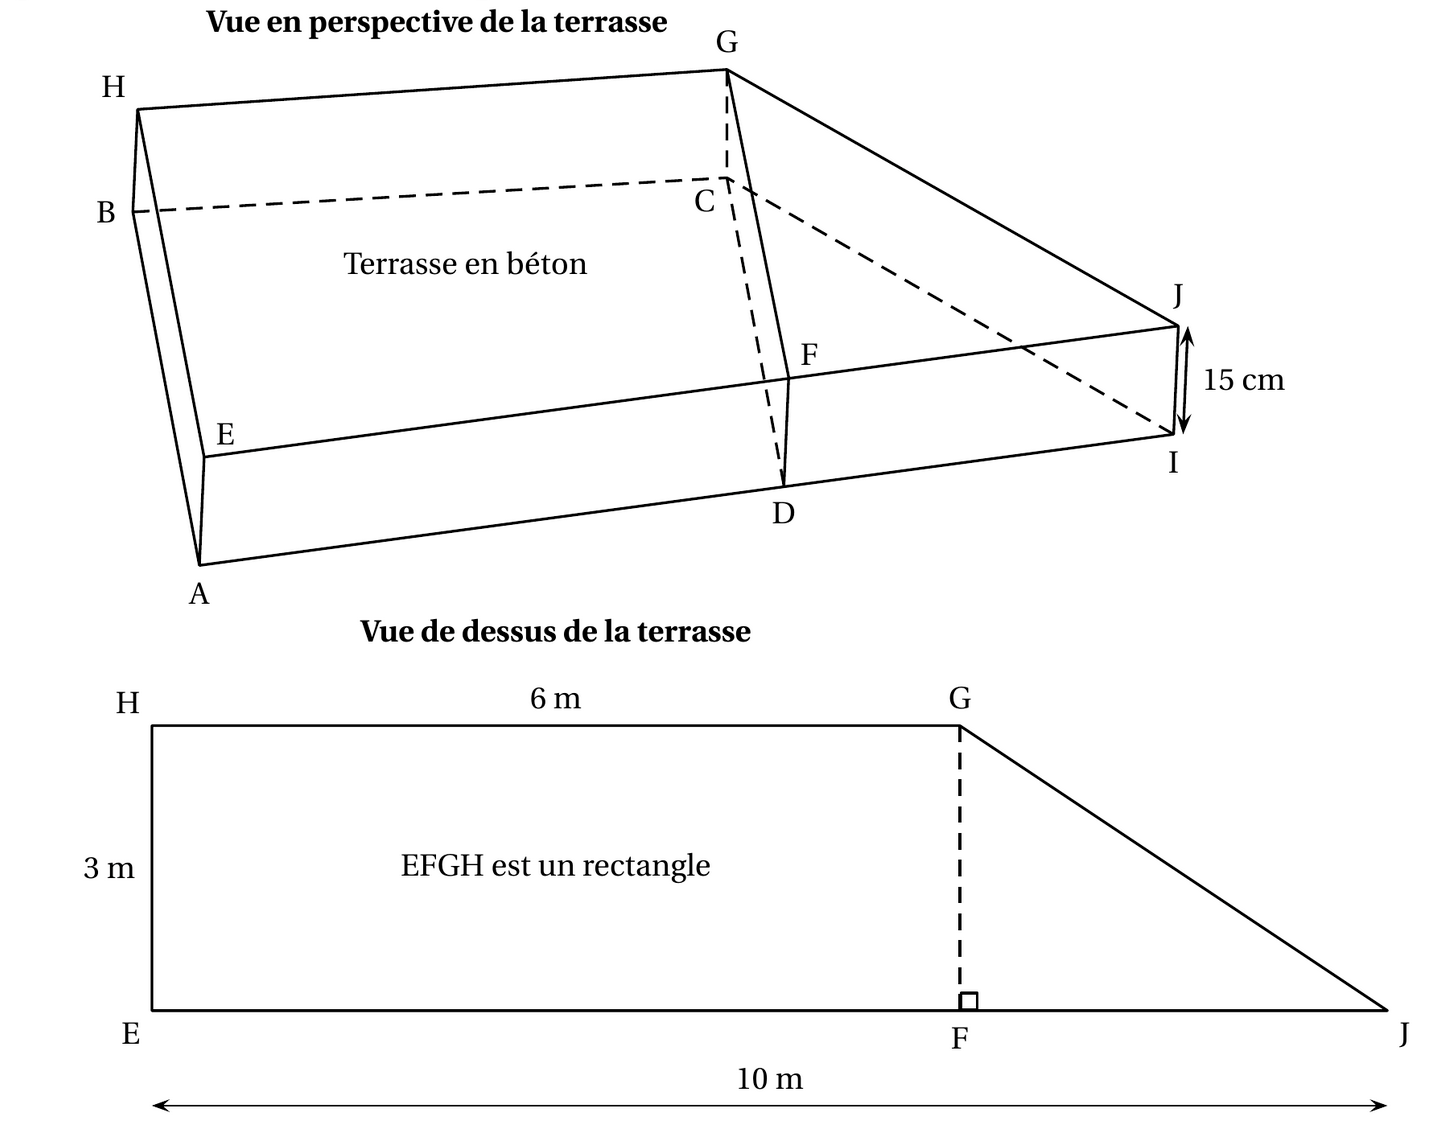
\includegraphics[scale=.7]{Figure}
\end{center} 

\begin{enumerate}
\item[1).] Montrer que FJ $= 4$~m.

\item[2).] Afin de pouvoir couler le béton, M. et M\up{me} Martin doivent délimiter la terrasse en installant des planches tout autour. Quelle longueur de planches doivent-ils acheter au minimum ?

\item[3).] M. et M\up{me} Martin souhaitent réaliser $4 \mathrm{~m}^{3}$ de béton.
	\begin{enumerate}
		\item Montrer que le volume de la terrasse est bien inférieur à $4 \mathrm{~m}^{3}$.

		\item Sachant que pour faire 1 m$^{3}$ de béton, il faut $250$~kg de ciment, quelle masse de ciment (en kg) doivent-ils acheter pour réaliser 4 m$^{3}$ de béton ?
		
		\item Pour faire du béton, on ajoute de l'eau à un mélange de ciment, de gravier et de sable.
Dans ce mélange, les masses de ciment - gravier - sable sont dans le ratio $2~:~ 7~:~5$.

Déterminer (en kg), la masse de gravier et la masse de sable nécessaires pour réaliser les 4 m$^{3}$ de béton.

	\end{enumerate}
	
\item[4).] M. et M\up{me} Martin souhaitent peindre la surface supérieure de leur terrasse.

À l'aide des documents 1, 2 et 3 , déterminer le type et le nombre de pots nécessaires pour effectuer ces travaux avec un coût minimum.

\medskip

\textbf{Document 1 :} Pots de peinture proposés

\begin{center}
\begin{tabular}{|c|c|c|}\cline { 2 - 3 }
\multicolumn{1}{c|}{} 		&Pot A 	& Pot B \\ \hline
Contenance (en litres) 	&5 		& 10 \\ \hline
Prix (en euros) 			&79,90 	& 129,90 \\ \hline
\end{tabular}
\end{center}

\textbf{Document 2 :} L'offre du mois : Moins 50\,\% sur le deuxième article identique.

\medskip

\textbf{Document 3 :}

Deux couches de peinture sont nécessaires. 1 litre de peinture permet de réaliser une couche de 5~m$^{2}$.
\end{enumerate}
\begin{center}
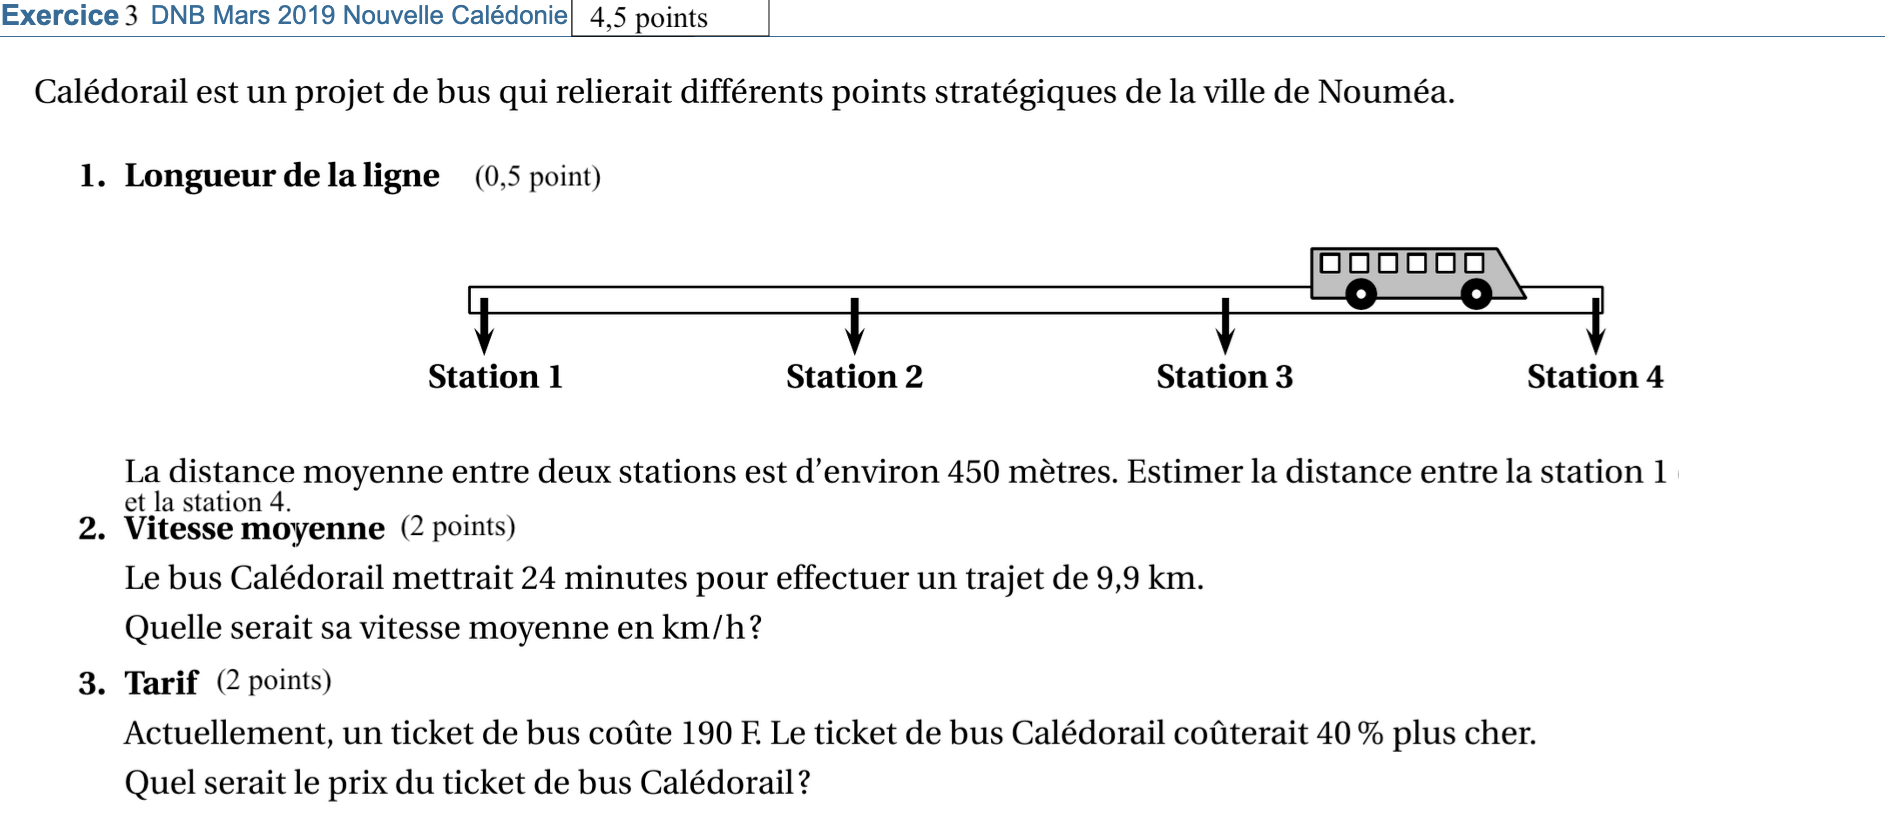
\includegraphics[scale=.65]{Train}
\end{center}


 	\end{document}
